\section{Experiment}
The present commissioning experiment was performed in 2020 at the FAIR Facility at GSI (Gesellschaft f\"ur Schwerionenforschung) in Darmstadt (Germany). The GSI Helmholtzzentrum für Schwerionenforschung operates a unique accelerator facility for heavy ions and focuses on several cutting-edge research fields. These include:\newline
\begin{enumerate}
\item \textbf{Nuclear Physics}: Studying the properties of atomic nuclei, exploring the forces that bind protons and neutrons, and investigating exotic nuclei far from stability.
\item \textbf{Hadron and Quark Matter}: Investigating the behavior of hadrons (particles made of quarks) and the state of matter under extreme conditions, such as those found in neutron stars or during the early universe.
\item \textbf{Atomic Physics}: Examining the structure and dynamics of atoms, including highly charged ions, to understand fundamental atomic interactions and refine quantum electrodynamics.
\item \textbf{Plasma Physics}: Creating and analyzing high-energy-density plasmas to simulate conditions found in stellar interiors and other astrophysical phenomena.
\item \textbf{Biophysics and Medical Research}: Exploring the effects of ion beams on biological systems for applications in cancer therapy, particularly using heavy ion therapy, and studying radiation protection for space missions.
\item \textbf{Materials Research}: Investigating the response of materials to high radiation doses to develop more resilient materials for use in various technologies, including nuclear reactors and space exploration.
\end{enumerate}
\subsection{GSI facility}
The GSI Helmholzzentrum f\"ur Schwerionenforschung located at Darmstadt has a long history of research.... tell something about the beginnnings, first really heavy elements found there.\newline
%Tell about the central apparatus: Linear Accelerator UNILAC, Ring Accelerator SIS 18, FRS,  and the different experimental halls, see: https://web.archive.org/web/20141222164000/https://www.gsi.de/en/research/accelerator_facility.htm?nr=%2Fproc%2Fself%2Fe
The GSI Helmholtzzenrum f\"ur Schwerionenforschung GmbH was founded in 1969 (as "Gesellschaft f\"ur Schwerionenforschung mbH) looks back on a successful research history. In the time between 1981 and 2010 six new  superheavy elements were discovered. \newline
In the medical research field GSI has developed advanced cancer therapy techniques using heavy ion beams which target tumors with high precision, minimizing damage to surrounding healthy tissues.\newline
Along with those groundbreaking discoveries in research the facility at GSI has always been an inspiring source of drive for new technologies.\newline
The key devices/apparatus which enable to carry out experiments with heavy ions at GSI are:
%cite from:
%https://www.gsi.de/en/researchaccelerators/accelerator_facility
important to mention: GSI is the only facility with heavy ions in the world
The starting point for the production of relativistic heavy ions at GSI is the ion source where ions are generated by stripping electrons off the shell of the atoms. Depending on the experimental needs the ion sources at GSI are able to produce ions of many different kinds of elements (up to Uranium).\newline
%cite here: https://www.gsi.de/en/researchaccelerators/accelerator_facility/ion_sources
On the first acceleration stage the stable primary ions are injected from the ion source into the UNIversal Linear Accelerator (UNILAC). On a length of 120 meters ions are accelerated up to maximum energy of 11.4 AMeV. The low energy beam is now injected into the ring accelerator SIS18 (Schwerionensynchotron 18). Here the ion beam is further accelerated up to 4.7 GeV/u (for protons) / 1 GeV/u (for Uranium). The magnets and  the ultra-high vacuum ($\sim$ $10^{-9}$ Pa) keep the ions well on their circular path (SIS18 has a circumference of 216 meters). For the production of rare heavy isotopes the primary ion beam from SIS18 can be impinged on a light nuclear target, e.g beryllium, the so called production target. These secondary beams of radioactive isotopes can be either stored in the experimental storage ring (ESR) for later use or transferred to the FRagment Separator (FRS). The FRS as a high-resolution magnetic spectrometer is capable to precisely select specific isotopes and to forward the desired beam of exotic relativistic nuclei to the various experiments or direct it to the ESR for later use.\newline
%cite here: https://www.gsi.de/en/researchaccelerators/accelerator_facility/ring_accelerator
\subsubsection{FAIR Project}
The FAIR (Facility for Antiproton and Ion Research) situated next to the GSI will be one of the most complex and largest accelerator facilities in the world. The construction of the superconducting ring accelerator SIS100 with a circumference of 1.1 km, storage rings and experiment sites begun in the summer of 2017. Commissioning is planned in 2025 (?). Early Science. Before the commmissioning of the ring accelerator SIS100 several prioritized experiments with large impact in the scientific world will take place in the newly built experimental halls, such as experiments with the R3BSetup in the High Energy Cave (HEC).\newline
 
\subsection{R3B Setup}
The R3B (Reactions with Relativistic Radioactive Beams) experiment in Cave C at the GSI Helmholtz Centre for Heavy Ion Research in Germany is a cutting-edge research experiment focused on the study of nuclear reactions and structure using high-energy radioactive ion beams. The experiment aims to investigate exotic nuclei far from stability, offering insights into the fundamental properties of nuclear matter, nucleosynthesis processes, and the forces governing nuclear interactions. A schematic overview of the R3B Setup can be seen in Figure blabla. \newline
The short living (neutron rich) isotopes are injected to the Cave C from the FRS, which preselects as mass spectrometer the isotopes of interest, and impinge on a fixed target. The R3B setup is designed for kinematically complete reaction studies. To fulfill this requirement the incoming ions are tracked and identified on an event-by-event basis by dedicated detectors in the FRS via time-of-flight and deltaE measurement techniques. Depending on the settings and composition of the incoming ion beam different type of reactions take place in the target area with a large variety of reaction products: heavy ions (as producs from fission/spallation reactions), neutrons, light charged particles and gamma rays. For the detection of gammas and light charged ions from reactions with the target the dedicated CALIFA calorimeter (see more in section blabla) and various tracking detectors are installed in the target region. The GLAD (GSI Large Acceptance Dipole) magnet, located at the center of the Cave C, acts as mass spectrometer for the forward boosted charged reaction residues. The magnetic rigidity of the charged reaction residues is measured by a combination tracking detectors and a time of flight wall after the GLAD magnet. This allows to identify the charged reaction residues and their momenta. For the detection of the neutrons, not deflected by the magnetic field of the GLAD magnet, the new array neutron detector (NeuLAND) is positioned after GLAD on the zero degree line with the incoming ion beam.\newline
The high flexibility of the R3B Setup, it can be operated with 
The combination of the large spectrum of incoming ion beams in a broad energy range provided by the FRS facility and the high flexibility of the R3B Setup with state of the art detectors for the specific physics-studies of interest makes it to an attractive play-ground for experimental astro-physics.\newline
\subsection{Detector Setup in S444 Commmissioning Experiment 2020}
The S444 Experiment (successor experiment of the FAIR Phase-0 program in 2019, ref to Lukas Ponnath Thesis) for the commissioning of the CALIFA Calorimeter in its final mechanical design took place in February 2020. The choice to operate with stable 12C primary beam with four beam energy settings - 400/550/650/800 AMeV  gave the opportunity to use it as preparation for the following up S467 experimental run with neutron-rich Ca isotopes as medium-heavy incoming beam. The detectors for positional tracking, charge identification and time measurement were provided by the SOFIA(Study on Fission with Aladin, make footnote that ALADIN was the precessor or GLAD) collaboration. These detectors are optimized for fission experiments with medium to heavy reaction fragments. As for the S444 experiment with primary 12C incoming beam no fission reaction with multiple heavy charged fragments is expected the Sofia detectors were adapted accordingly (e.g. only one of the four sections of the Twin-Music Ionisation chamber was operated, see more in chapter Twin).\newline
For this commissioning experiment most detectors and parts of the setup were operated in air. The target chamber was evacuated by gaseous helium at room temperature as well as the GLAD magnet. The fact that the ions interact with particles in air causes ancular straggling in the flightpath reconstruction and can limit the resultion of reconstruced momenta from the reaction on the target\cite{AbedonHymanThomas2003}.\newline  
\subsubsection{Multi Wire Proportional Chambers (MWPC)}\label{sec_mwpcs}
The positional tracking of the incoming ions as well as the charged reaction products were perfomed by using Multi Wire Proportional Chambers (MWPC). A MWPC operates on the principle of proportional counters that are arranged side by side in a plane, thereby providing spatial resolution for particle radiation. The multi wire proportional chambers were developed in late 1960s by George Charpak\footnote{George Charpak received the Nobel Prize in Physics in 1992 for his invention and development of particle detectors, in particular, the multiwire proportional chambers.} at CERN\cite{charpak1968use}.\newline
The MWPC operates in the same way as aligned proportional counters with the difference of not having dividing walls between the anode wires. This reduces the material budget, hence improving the spatial resolution and reducing reactions with the detected particle.\newline
In the general design the  MWCP is made up of a plane of anode wires enclosed between two cathode planes which are aligned parallel or vertical to the anode wires. Depending on the beam conditions the anode wires are set to high voltage ($\sim$ 1100 V) while the cathode planes are grounded.\newline
The volume between the two cathode planes is filled by a gas mixture of 84\% Argon and 16\% CO\textsubscript{2}. The decision of the gas mixture is driven by a balaced ratio between amplification and quenching propreties of the gas.\newline
When a charged particle passes through the detector it ionizes the gas. Primary electrons are created followed by a secondary ionization via electron avalanche. The electron avalanche drifts towards the wires (anodes) while the positive ions drift towards the grounded cathode planes. As the MWPCs are operated in the proportional region, the number of created electrons/ions is proportional to the initial ionization. Instead of reading out the signal from the wires it is read out from the strips of the cathode plane. This improves the position resulution in case the cathode planes are aligned prependicular to the wires. In case multiple (neighboring) strips give signal the signal distribution over the strips is anayzed and fitted to provide the position information.\newline
In the R3B setup for the S444 experiment four MWPCs were installed:\newline
\begin{enumerate}
\item MWPC0: right at the beginning of the beam entrance in Cave C, $184$ cm upstream to the target position to detect x- and y positions of the incoming ions.
\item MWPC1: $88$ cm downstream to the target for positional tracking in x and y of the outgoing reaction fragment
\item MWPC2: $154$ cm downsteram also for positional tracking of the fragment
\item MWPC3: after the GLAD magnet. The x position of this detector gives the information about the magnetic rigidity of the reaction fragment.  %todo: find out position relative to Sofia TOFW
\end{enumerate}
Despite having the same mode of operation, they slightly differ in their construction design and positional resolution. For the technical specifications of the individual MWPCs, see table \ref{table:mwpcs_tecs}.
\begin{table}[h]
    \centering
    %\begin{tabular}{|l|l|}
    \begin{tabular}{cc}
        %hline
        \multicolumn{2}{c}{\textbf{Common MWPC Settings}} \\ 
        \hline
        Gas & 84\% Ar, 16\% CO$_2$ \\ 
        %%hline
        Windows & Mylar\textregistered \\ 
        %%hline
        Anode wires voltage & 1100 V \\ 
        %%hline
        Cathode planes voltage & Ground \\ 
        %%hline
        Wire pitch & 2.5 mm \\ 
        %%hline
	Wire diameter & 5 $\mu$m\\
        %%hline
        Width of X pads & 3.125 mm \\ 
        \hline
	%\hspace
	\vspace{2\baselineskip}\\
        \multicolumn{2}{c}{\textbf{MWPC0}} \\ 
        \hline
	X pads & 64 pads, vertically segmented into two equal parts \\
	Y pads & 64 pads, horizontally segmented (3.125 mm width)\\
	Active surface & 200 $\times$ 200 mm$^2$ \\
        \hline
	\vspace{2\baselineskip}\\
	%\hspace
        \multicolumn{2}{c}{\textbf{MWPC1 \& MWPC2}} \\ 
        \hline
	X pads & 64 pads, vertically segmented into two equal parts \\
	Y pads & 40 pads (5 mm width), horizontally segmented\\
	Active surface & 200 $\times$ 200 mm$^2$ \\
	\hline
	\vspace{2\baselineskip}\\
	%\hspace
        \multicolumn{2}{c}{\textbf{MWPC3}} \\ 
	X pads & 288 pads \\
	Y pads & 120 pads (5 mm width) \\
	Active surface & 900 $\times$ 600 mm$^2$ \\
	\hline
	%todo: check again with are segmented to equal parts and which not...
    \end{tabular}
    \caption{SOFIA MWPCs - Technical specifications}
	\label{table:mwpcs_tecs}
\end{table}
Still to do: put in plot with potential field of mwpcs and one with crossign charged particle.
\subsubsection{Ionisation Chambers - R3BMusic/TWIM Music}
For the S444 experiment at R3B two types of \textbf{m}ulti \textbf{s}ampling \textbf{i}onisation \textbf{c}hambers (MUSICs) were installed: the R3B MUSIC, centered 153 cm upstream to the target, and the TWIN-MUSIC, 132 cm downstream to the target. Like the MWPCs (see \ref{sec_mwpcs}) the ionisation chambers are gas-filled detectors for tracking down charged particles. While MWPCs consist only of a few mm of active gaseous volume, the ionsiation chambers have an expanded gaseous volume which allows to make precise energy loss measurements from the ionisation process of the gas. The multi sampling ionsiation chambers consist of a cathode plane and an anode plane, consisting of multiple anode strips. When a charged particle crosses the chamber the gas gets ionized and the created electrons and ions are separated by the strong electric field. While the ions drift towards the cathode plane the electons move to the anodes where each anode is read out separately. Since the energy loss of the passing through particle is proportional to the square of its charge ($\Delta E \sim Z^2$) the signal from the anodes allow to precisely measure the charge of the particle. Moreover multi-sampling ionisation chambers measure the drift time of the electrons created during the ionisation process  on each anode (compared to one or more reference anodes). Assuming a constant electron drift velocity ($\sim 40 mm/\mu s$) over the gaseous volume the time information of each anode signal can be used to reconstruct the x-position of the passing through paricle).\newline
\textbf{R3B MUSIC}\newline
The R3B MUSIC, installed 153 cm upstream to the target, is used to measure both the  charge of of the incoming ion before impinging on the target and the angle of the particle's trajectory. The detector has an active gaseous dimension of 20 x 20 x 40 $cm^3$, confined on one side by a cathode plane and on the other side by an anode plane consisting of 10 anodes ( 8 readout anodes and 2 screen anodes). For the technical specifications, see table \ref{table:r3bmusic_tecs}. \newline
\begin{table}[h!]
    \centering
    \begin{tabular}{ll}
    %\begin{tabular}{cc}
        \hline
        \textbf{Dimensions} & \\ 
	Detector dimension: & 51 x 54 x 53 cm$^3$ \\ 
	Active dimension: & 20 x 20 x 40 cm$^3$\\
	Dimension of one anode:& 20 x 20 x 5 cm$^3$\\
	Dimension of one screen anode:& 20 x 20 x 2 cm$^3$\\
	\textbf{Gas} &\\
	P75 (Ar 25\%, CH4 75\%) \\
	\textbf{Voltage} & \\
	Cathode (left to beam direction): &  $-(2-6)$kV \\
	Anode (right to beam direction): & $+300$V \\
	\textbf{Resoultions} & \\
	still to do! & \\
	\hline
    \end{tabular}
    \caption{R3B MUSIC - Technical specifications}
	\label{table:r3bmusic_tecs}
\end{table}
\newline
\textbf{TWIN MUSIC}\newline
The TWIN MUSIC is a double ionisation chamber with one central cathode plane and two independent drift volumes and anode planes on each side. Each of the anode planes consists of 16 anodes for readout plus two screen anodes. Furthermore each anode is again segmented into up/down which splits the detector into four dedicated sections. As the TWIN MUSIC is placed 132 cm downstream to the target it is employed to measure charge and angular direction of the outgoing medium-to-heavy fragments. The detector was in particular designed for fission experiments where two or more fission fragments are created. If each fragment is flying through one of the four sections ( which is mostly the case due to momentum conservation rules) charge and angle of each fragment can be measured independently.\newline
To fulfill the required permanence of the field in both extended gaseous volumes (of dimension 11x22x40 $cm^3$) a Frisch grid is located 3 mm from the anode planes. The Frisch grid is metal mesh grid that shields the anode from the movement of ions produced during ionization process in the chamber ensuring that only the electrons that reach the anode contribute to the signal. Additionally,the shielding of the anodes by the Frisch grid account for the fast rise time of the signal at the anodes which diminishes pile-up effects and makes the detector high beam-rate capable (up to 100kHz). Further technical specifications you can find in table (bla bla)
\newline
\begin{table}[h!]
    \centering
    \begin{tabular}{ll}
    %\begin{tabular}{cc}
        \hline
        \textbf{Dimensions} & \\ 
	Detector dimension: & 43 x48 x55 cm$^3$ \\ 
	Active dimension: & two halves each  11x22x40 cm$^3$\\
	Distance central cathode - Frish grid: & 11 cm\\
	Distance Frish grid from anode planes: & 3mm\\ %todo 11cm +3 mm = 11cm?!?
	\textbf{Gas} &\\
	CH4 [79\%], Ar [20\%] and CO2 [1\%] \\
	\textbf{Voltage} & \\
	Central cathode: &  $-(2-6)$kV \\
	Anode planes: & $+600$V \\
	Frish Grid: & $+250$V\\
	\textbf{Resoultions} & \\
	$\Delta E / E$ & $< 5$\% FWHM, total < 2\% FWHM \\
	$\Delta X$ & $< 40 \mu$m\\
	\hline
    \end{tabular}
    \caption{TWIN MUSIC - Technical specifications, see also \cite{martin2021fission}}
	\label{table:twin_tecs}
\end{table}
\newline
    

\subsubsection{Sofia Start Detector}
The SOFIA Start detector is positioned right after the R3B Music ionisation chamber and gives a time reference for the incoming ion. It is a 1 mm thin scintillating plastic blade attached with a photo multiplier tube on each side. The scintillator light from excitation of the incoming ions produce a clear signal on both photomultiplier tubes used for the time measurement: \[t_{start} = 0.5 \cdot (t_{left}+t_{right}) \]\newline
To shield the plastic detector from daylight it is wrapped in mylar foil (300$\mu$m thickness).
\subsubsection{GLAD Magnet}
The \textbf{G}SI \textbf{L}arge \textbf{A}cceptance zero degree superconducting \textbf{D}ipole magnet \textbf{GLAD} sits in the center of the R3B Setup in the cave C hall\ref{fig:GLAD}. With an adjustable field integral up to 5 Tm it has a high acceptance range in magnetic rigidity which is crucial for the identification of highly asymmetric reaction fragments. The homogeneous magnetic field in GLAD allows to achieve momentum resolutions $\Delta p$ /p of 10$^-3$ in combination with the dedicated tracking system.\newline
The large opening angle of $\pm$ 80 mrad makes the GLAD magnet highly transmissive for evaporated or scattered neutrons in the reaction process which will be subsequentely detected in the NeuLAND detector.\newline
The default bending angle of the beam with respect to the beam line was set to 18$^{\circ}$. Herefore the currents where adjusted according to the beam energy:\newline
\newenvironment{tight_enumerate}{
\begin{enumerate}
  \setlength{\itemsep}{0pt}
  \setlength{\parskip}{0pt}
}{\end{enumerate}}
\begin{tight_enumerate}
\item 400 AMeV beam: 1444 Ampere
\item 550 AMeV beam: 1778 Ampere
\item 650 AMeV beam: 1957 Ampere
\item 800 AMeV beam: 2223 Ampere
\end{tight_enumerate}
\begin{figure}[htpb]
    \centering
    \includegraphics[width=\textwidth,height=6cm,keepaspectratio=true]{Figures/glad_magnet.jpg}
    \caption{
    Upstream view of GLAD magnet in the center of Cave C after installation in February 2016. Picture from \cite{wiki:GLAD} 
    }
    \label{fig:GLAD}
\end{figure}
\subsubsection{CALIFA Calorimeter}
The \textbf{CAL}orimeter for \textbf{I}n \textbf{F}light detection of $\gamma$-rays and high energy charged p\textbf{A}rticles, CALIFA, is one of the main detector components of the R3B setup. It surrounds the target area and covers the full azimuthal range and a polar angular acceptance from 7$^{\circ}$ up to 140$^{\circ}$ in the target region. The calorimeter serves for the detection of gamma rays in the energy region 100 keV $\lesssim$ E\textunderscore$\gamma$ $\lesssim$ 30 MeV and light charged particles, mostly protons, up to E\textunderscore p $\lesssim$ 700 MeV. To fulfill the demands requested by the different experimental campaigns an energy resoultion of $\frac{\Delta E}{E}$(@1MeV) $\sim$ 6\% in the gamma-ray energy regime $\frac{\Delta E}{E}$(@100MeV) $\sim$ 1 \% in the proton range regime is required.\newline
%
%The CALIFA calorimeter, with its 2528 CsI scintillation crystals in its final design, is a key detector
%in quasi-free-scattering experiments at R3B. Covering the full azimuthal range and having a polar
%angular acceptance from 22° up to 89° in the target region already now it allows to detect both the
%two coincident protons from the quasi-free-scattering process and emitted γ-rays from de-excitation
%of the remaining nucleus with high angular resolution and precise Doppler correction.
\textbf{Geometry}\newline

The CALIFA detector is a highly segmented detector with more than 2500 CsI crystals installed in the final design. Since experiments in the R3B setup operate in relativistic kinematics both the incoming ions as well as the the measured particles originating from reactions inside the source experience relativistic effects, more precisely the so called relativistic Doppler effect. The emitted gammas and protons are not isotropically distributed around the source region but are boosted in forward direction. Moreover, the energy measured in the lab frame is different from the kinetic energy in the rest frame of the incoming ion.\newline
%find formula for theta relativistic for massive/massless particles

The relativistic Doppler effect has a huge impact on the geometric design and requirements of CALIFA. Herefore the detector was subdivided into three polar angle ranges\ref{fig:califa_sec}:
\begin{figure}[htpb]
    \centering
    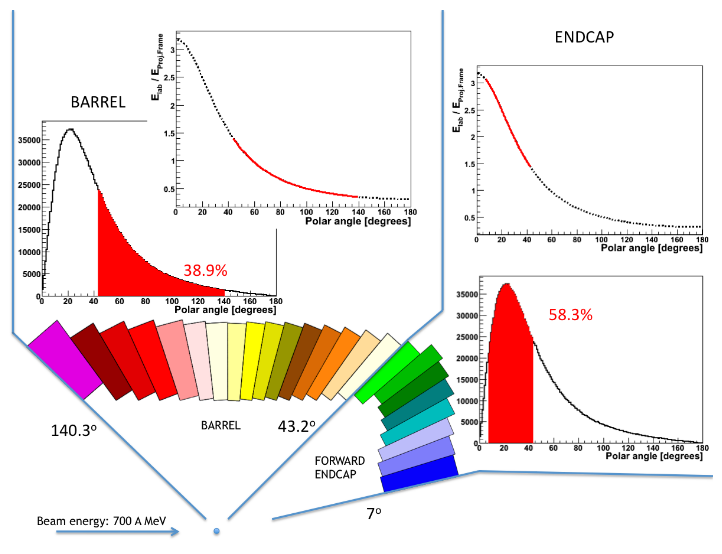
\includegraphics[width=\textwidth,height=10cm,keepaspectratio=true]{Figures/califa_section_overview.png}
    \caption{
    Schematic view of the Barrel and Endcap(iPhos and CEPA) segments of CALIFA and the according angular and energy distribution of emitted $\gamma$ rays (monoenergetic in the projectile frame at beam energy of 700 AMeV). From \cite{tdr:barrel}
    }
    \label{fig:califa_sec}
\end{figure}

\begin{enumerate}
\item[$\blacksquare$] $7^{\circ} \leq \theta \leq 19^{\circ}$ - CEPA (CALIFA Endcap Phoswich Array): The most forward segment consists of 96 CsI(Tl) crystals. Due to the aforementioned rel. Doppler effect this area will have the highest intensities and energies. For high beam energies most of the particles will not be stopped inside the crystal and will escape as "punch-throughs". Despite the "punch-through" ions deposit only a fraction of their kinetic energy ($\Delta E$) in CALIFA it is possible to reconstruct the initial energy of the particle \footnote{This is done by exploiting the distinct scintillation components of CsI, see more in chapter 5 of \cite{Bendel:98055}}. In CEPA crystals with a length of 15 cm are used and cover each a polar angle of $\approx$ 2$^{\circ}$. This finer segmentation in polar angular range has the benefit to compensate for the high rate.     
\item[$\blacksquare$] $19^{\circ} \leq \theta \leq 43^{\circ}$ - Intristic Phoswich (iPhos): In conjunction with the CEPA, the iPhos region forms a part of the CALIFA Endcap. The iPhos region is, same as for the CEPA, affected by hight rates. Protons reaching this region have high kinetic energies ($E_{kin,p} \leq 600 MeV$) and herefore a large fraction of "punch-throughs" are expected. In the iPhos region 480 CsI(Tl) crystals with a length of 22 cm\footnote{To fully stop protons with $E_{kin,p} \approx 600 AMeV$ crystals with a lenght of 60 cm would be needed. Such long crystals would have multiple drawbacks: reduced energy resolution due to worse scintillator light transport, enhanced nuclear reactions inside the crystals and challenging demands on stability of the detector holding structure} are installed and cover each a polar angle of $\approx$ 3$^{\circ}$.(For more information see Endcap TDR:\cite{tdr:endcap}).
\item[$\blacksquare$] $43^{\circ} \leq \theta \leq 140^{\circ}$ - Barrel: This segment covers the region where the lowest rates and energies are expected. The Barrel region contains 1952 CsI(Tl) crystals, due to the large polar angular coverage and the requirement of Doppler correction via angle measurement. The most forward crystals have a length of 22 cm (which allow to stop protons with $E_{kin,p} \leq 315 MeV$). This length is reduced down to 12 cm for the most backward crystals (For more information see Barrel TDR:\cite{tdr:barrel}).   
\end{enumerate}
The crystals are arranged in carbon fibre alveoli with a nominal wall thickness of 230 $\mu m$\cite{tdr:barrel} that provide a support structure for the crystals and keep the material budged as low as possible. The alveoli in turn are hold and covered by individual aluminium tiles. The volume enclosed by the alveoli and the aluminium tiles is flooded with nitrogen to keep humidity low on the surface of the crystals. For a sufficient suspension of the aluminium cover a robust external holding structure was designed.\newline
\begin{figure}
     \centering
     \begin{subfigure}[b]{0.4\textwidth}
         \centering
         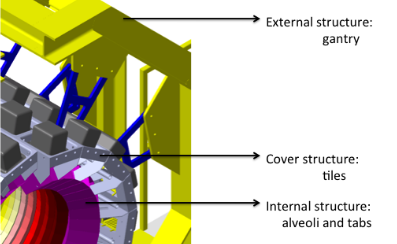
\includegraphics[width=\textwidth]{Figures/califa_inner_outer_structure.png}
         \caption{Zoomed view between inner and outer strucure layers, from \cite{tdr:barrel}. The black boxes symbolize the preamplifiers, which are directly mounted on the aluminium tiles.}
         \label{fig:califa_frame_zoom}
     \end{subfigure}
     \hfill
     \begin{subfigure}[b]{0.4\textwidth}
         \centering
         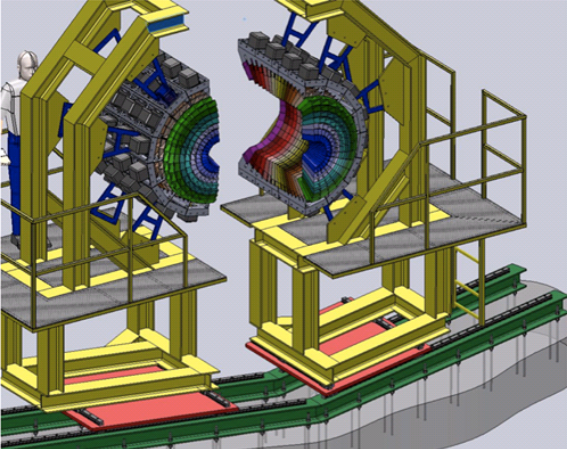
\includegraphics[width=\textwidth]{Figures/califa_frame.png}
         \caption{Artistic view of the outer support structures, from \cite{tdr:endcap}. For better access to the target area the detector infrastructure is split into two halves, the left side commonly referred as "Messel" and the right side as "Wixhausen" (in-beam-view).}
         \label{fig:califa_frame}
     \end{subfigure}
     \hfill
        \caption{CALIFA internal and external holding structure}
        \label{fig:califa_holding_structure}
\end{figure}
In 2019 CALIFA was for the first time integrated into the R3B setup in form of the CALIFA demonstrator, a prototype consisting of seven mechanically separate petals, each of it containing a set of 64 crystals.\newline
At the end of 2019 the CALIFA frame in its final design was installed and the forward barrel part ($43^{\circ} \leq \theta \leq 90^{\circ}$ and full azimuthal coverage) was equipped with 1024 crystals.\newline
For the S444 and the S467 experiment in 2020 CALIFA was equipped with 180 more crystals in the iPhos region ($19^{\circ} \leq \theta \leq 43^{\circ}$) which correspons a coreage of 37.5 \% in azimuthal angle for that region. Right before the S455 fissioning experiment \cite{grana2023fission} the full installation of the iPhos region was completed.\newline
In February 2024 the full CEPA region ($7^{\circ} \leq \theta \leq 19^{\circ}$) with 96 crystals was commissioned for the first time together with a new equipped part of the backward barrel ($90^{\circ} \leq \theta \leq 102.5^{\circ}$, 128 crystals).\newline   
\textbf{Energy and particle reconstruction with CsI scintillator crystals}\newline
Scintillator material, as caesium iodide doped with thallium (CsI(Tl)), is widely used in experimental physics to detect ioinizing radiation from $\gamma$- rays or charged particles. The energy from the incoming radiation excites the electrons in the CsI crystal from their ground state to higher energy levels (excited states). The deexictation, followed by photon emission (scintillation light), ocurrs via various complex mechanisms, not all of them completely understood yet (for more information see TODO:references!). The efficiency and properties of the scintillation process can be fine-tuned by doping CsI with small amounts of other materials, such as thallium. Thallium-doped Cesium Iodide produces light with a peak emission around 550 nm (green light) and has high light output\footnote{The light output per MeV deposited energy in CsI(Tl), measured in \cite{holl1988measurement}, resulted in  $5.2\cdot10^{4}$ (scintillation) photons/MeV.}. The high density of CsI with 4.51 g/cm$^3$ makes it to an optimal scintillator material to efficiently absorb $\gamma$- rays and other high-energy particles. Moreover the CsI(Tl) crystal is well transparent to its own scintillation light, which is essential for the detection of the scintillator light. CsI(Tl) crystals are in addition relatively robust compared to other crystals and only slightly hygroscopic making them suitable for long-term use in experimental setups.\newline
In a first approximation, the total amount of emitted light is proportional to the energy deposited in the scintillator. For $\gamma$ -rays this is valid for E$_{\gamma} \gtrsim 400 keV$\cite{syntfeld2007non}. However, for charged particles significant deviations from linearity are observed, a so called "$quenching$"(TODO: add here more information, also the thesis of Max Winkel).\newline
Although the the energy calibration of CsI(Tl) crystals for charged particles is challenging, CsI(Tl) as such  has the benefical property of having a complex time dependend light emission consisting of two distinct exponential components. The time dependend light emission response of CsI(Tl) $L(t)$ can be approximated as:
\begin{equation}
L(t) = \frac{N_f}{\tau_s} exp(-\frac{t}{\tau_f}) + \frac{N_s}{\tau_s} exp(-\frac{t}{\tau_s})
\end{equation}
Where $N_{f}$ is the amplitude of the fast component and $N_{s}$ the amplitude of the slow component. Accordingly $\tau_{f}$ the life time of the fast component ($\tau_{f} \approx 650-770 ns$ ) and $\tau_{s}$ the lifetime of the slow component ($\tau_{s} \approx 3.2 - 3.5\mu s$). It has been found that the proportion between the two components is energy and particle dependend. This proprety can be used to identify isotopes by extracting the $N_{f}$ and $N_{s}$ values from pulse shape anaylsis (PSA) on the according light emission response\footnote{The method has been implemented in the CALIFA Firmware as $Quick Particle Identification -QPID$. For more information see \cite{winkel2011implementierung} and \cite{winkel2016komplexe}}.  
TODO: put in a picture of nf vs ns an one with the scintillation light impulse\newline
%last can be found in paper : A method for the intrinsic calibration of CsI(Tl) detectors,D.V. Kamanin
%really brief description of how CsI works, and why we have chosen this material
%really brief how energy is reconstructed with PSA
%the two(or even three) light components to make PID
\textbf{From scintillator light to electrical signal}\newline
The scintillator light produced by the ionisation processes  has first to be transported to the back-end of the crystal. The optimum design has been determined to be frustrum-shaped crystals, wrapped into enhanced specular reflector (ESR) foil which provides excellent reflectivity. Finally at the backside of the crystals a large area avalance photodiode (LAAPD) is attached\footnote{Detailed information about the crystal wrapping and LAAPD gluing can be found in this work:\cite{hartigevolution}}. Avalanche photodiodes have the same working principle as photodiodes to convert (scintillator) light into electricity. As a result of an additional highly doted p-layer a region with very high field is formed which accounts for amplification factors up to $\approx$ 100.\newline
For the next amplification step the  electric signal is forwarded via thin ribbon cables to the back end of the preamplifiers from Mesytec\cite{mesytec-home} which can serve up to 32 input channels. For CALIFA two general types of peramplifiers are in use:
\begin{enumerate}
\item Dual Range (DR) Preamplifiers: They are used in the iPhos and CEPA region where both high energetic protons as well as gammas are expected. They cover two amplification ranges in parallel: the $gamma \enspace range$ with low input signal and high amplification and the $proton \enspace range$ with high input signal with low amplification. Following from this they have 64 channel differential signal output.
\item Single Range (SR) Preamplifiers: In the Barrel region, where mostly $\gamma$ rays are expected, only one amplification range is needed. Depending on the experimental demands these preamplifiers can be switched to $gamma$ or $proton \enspace range$. These peamplifiers have a 32 channel differential signal output.
\end{enumerate}
The fall time for the preamplifiers $\tau_{RC}$ has been chosen to $\approx$ 35 $\mu$s. This is a trade-off between the ballistic deficit on one side (reduction of the signal amplitude due to low $\tau_{RC}$, see also \cite{winkel2011implementierung}, chapter 3.4.5) and rate capability (restricted by large $\tau_{RC}$ value) on the other side.\newline
The differential signal output of the preamplifiers is then transmitted over shielded and twisted line pairs to the input of the FEBEX Addon Boards (FAB) for further processing.\newline
\textbf{Signal Processing and readout system}\newline
The central hardware module for the signal processing in CALIFA is the FEBEX 3B Module (Front End Board with optical link EXtension\cite{febex-tec}). Attached on it is a so-called AddOn board developed by TUM. The signal from the preamplifier gets here first filtered by a low pass two pole bessel filter ($f_{c} \approx 25 MHz$). Furthermore, since the input of the FEBEX ADCs cover a range of $\pm$ 0.9 V while the signal output from the preamplifier only has one polarity, an offset to the signal is applied to use the full range of the ADCs. The signal from the ADCs is read out continuously on the FEBEX card and split up into two branches:\newline
\begin{enumerate}
\item Fast/trigger branch:
\item Slow branch:
\end{enumerate}

%think about....
\subsubsection{Sofia Time of Flight Wall}
The Sofia Time of Flight Wall (or "Stop detector") is positioned at the very end of the experiment setup at approximately 6.6 m distance from the target position. It consists of a plane of 28 vertically aligned scintillator bars, each of dimension 32x600x5 mm. The scintillator plastics are numbered from 0 to 28 from left to right (when looking in beam direction). The time of flight of the ions between Start and ToFW can be measured by substracting the time measurement of  the Start detector from the ToFW. The combined resolution of the Start and TOFW detector is at 40 ps, for an average time of flight of 30 ns\cite{martin2021fission}. For the technical specifications of the Sofia ToFW, see table \ref{table:sof_tofw_tecs} and reference \cite{bail2011time}.
\begin{figure}
\begin{floatrow}
%\includegraphics[width=\textwidth,height=6cm,keepaspectratio=true]{Figures/sof_tofw.png}{
% \caption{Sofia TofW}%
% \label{fig:sof_tofw}
%}
\ffigbox{%
  \includegraphics[width=\textwidth,height=6cm,keepaspectratio=true]{Figures/sof_tofw.png}%
}{%
  \caption{Sofia ToFW in Cave C, from \cite{martin2021fission}.}%
}
\capbtabbox{%
  \begin{tabular}{cc}\hline 
  Plastic & EJ-232, no quencher \\ 
  Plastic dimensions & 5x32x600 mm$^3$ \\
  Detector dimension & 5x900x600 mm$^3$ (28 plastics) \\ 
  Photo-multiplier tubes &  Hamamatsu 6533 and 10580 \\
  Total number of PMTs & 56 (two per plastic - top and bottom) \\ \hline 
  \end{tabular}
}{%
  \caption{Sofia ToFW - Technical specifications}%
  \label{table:sof_tofw_tecs}
}
\end{floatrow}
\end{figure}

\subsubsection{NeuLAND Detector}
For the detection of knocked-out or evaporated neutrons the \textbf{N}ew \textbf{L}arge-\textbf{A}rea \textbf{N}eutron \textbf{D}etector (\textbf{NeuLAND}) is installed at zero degrees after GLAD. In its final design it will consist of 30 double planes with 100 plastic scintillators of size 5x5x250 cm$^3$ providing an active detector surface of 2.5x2.5 m$^2$ and thickness of 3m. Its high detection efficiency, a time resolution of $\sigma_t \le 150 ps$ and a mulit-neutron efficiency of 50\% to 70\% for four-neutron events are crucial detector features for complete kinematics experiments at R3B. For more detailed information, see \cite{boretzky2021neuland} and \cite{boretzky2014neuland}.\newline
For the S444 commissioning experiment in 2020 eight double-planes of the NeuLAND detector have been used. 

\subsubsection{Calibration of the Detector Systems}



